\newpage
\subsection{Actividad 7}
Trazar el lugar de las raices discreto en $z$ del sistema
servomotor de posición con \textsc{rltool} y situar los polos en bucle
cerrado para $k_a=1$, $k_a=10$ y calcular los valores de la ganancia
critica para el caso de que el controlador PID discreto sea una
ganancia $k_a$, comentando los resultados.

\begin{tcolorbox}[sharp corners, colframe=bluebox, title= Polos en
  bucle cerrado.,breakable = unlimited]
  $>>>$ rltool(Gposicionz)\\
  \vspace*{0.35em}
  \mkanscode{
\begin{figure}[H]
  \centering
  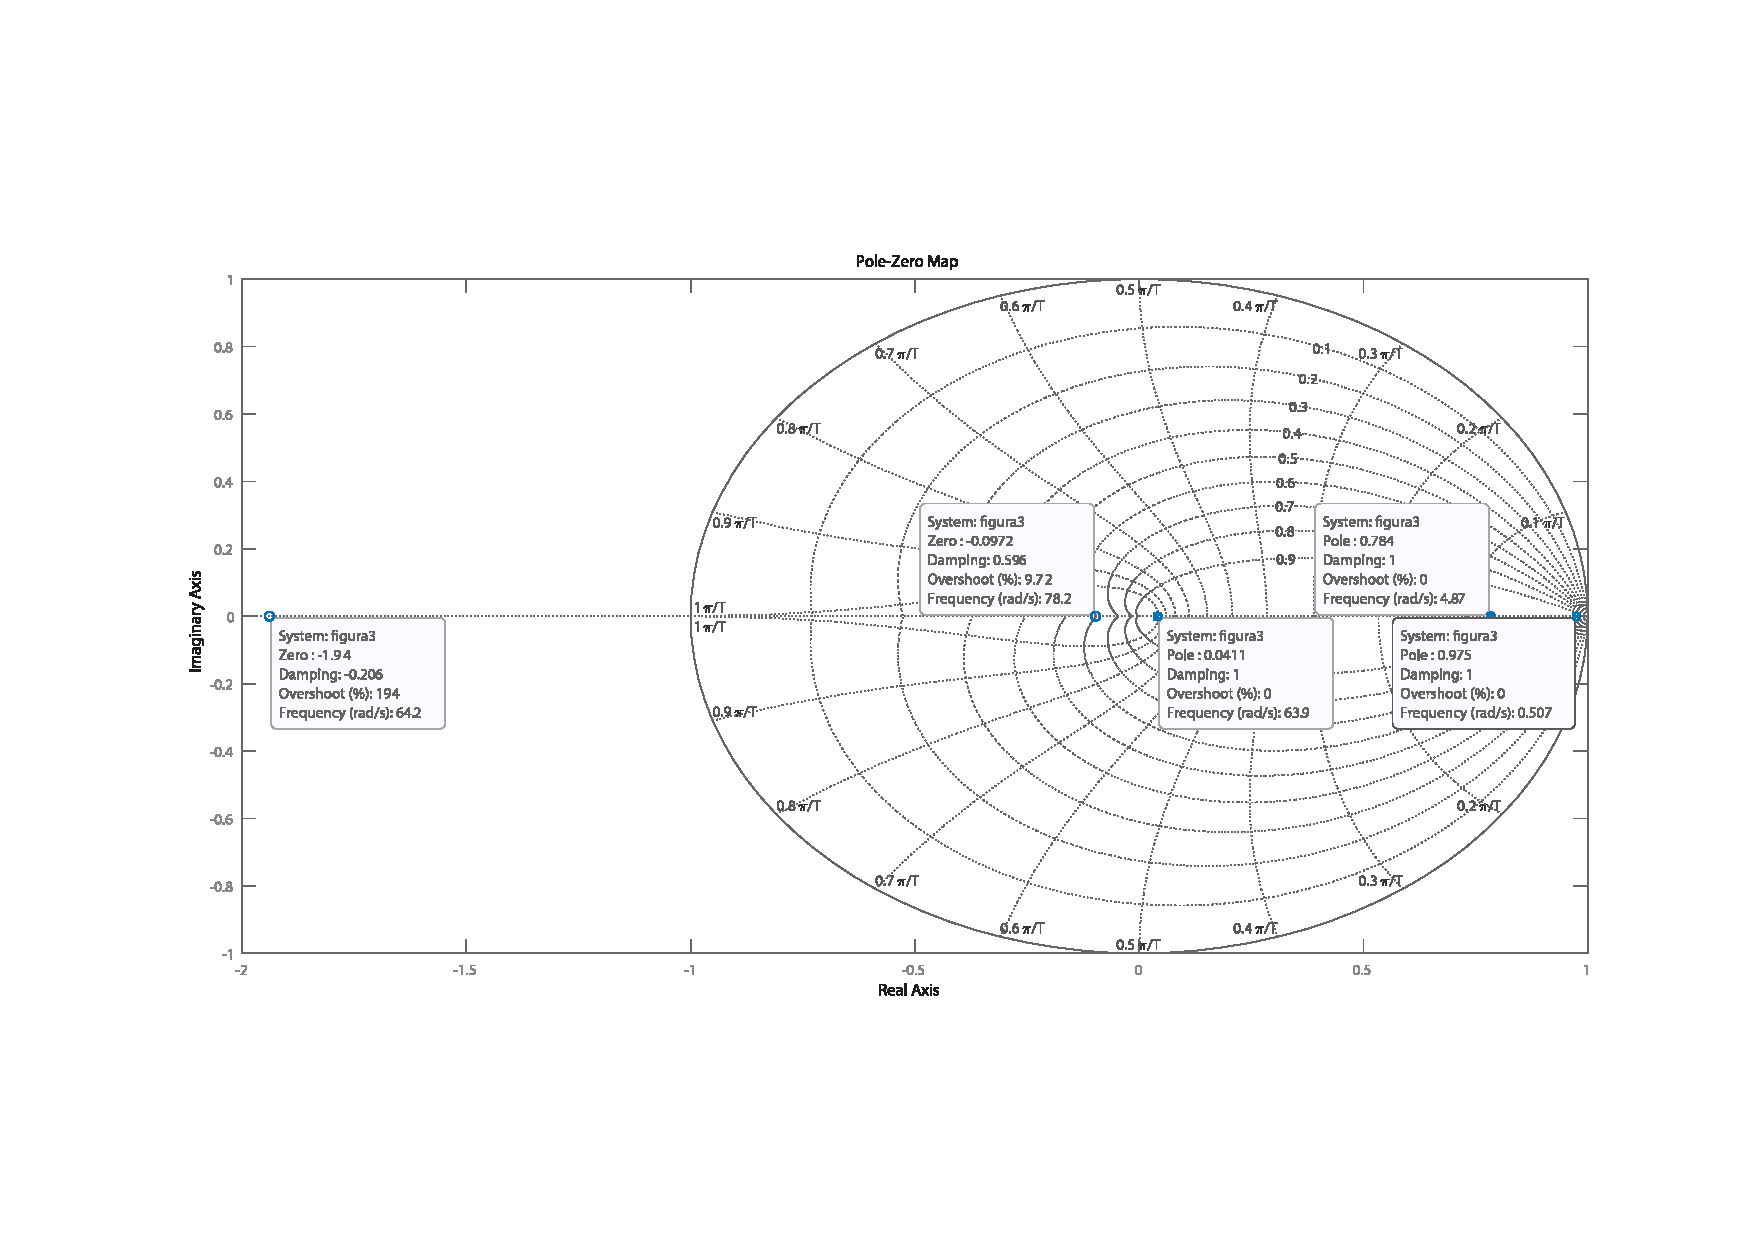
\includegraphics[clip, trim=3cm 4cm 2.8cm 4cm,
  scale=0.48]{images/figura 3.pdf}
  % izquierda,abajo,derecha,arriba
  \caption{Polos en bucle cerrado $k_a = 1$.}
    \label{fig:figura 3}
\end{figure}
}
  \mkanscode{
\begin{figure}[H]
  \centering
  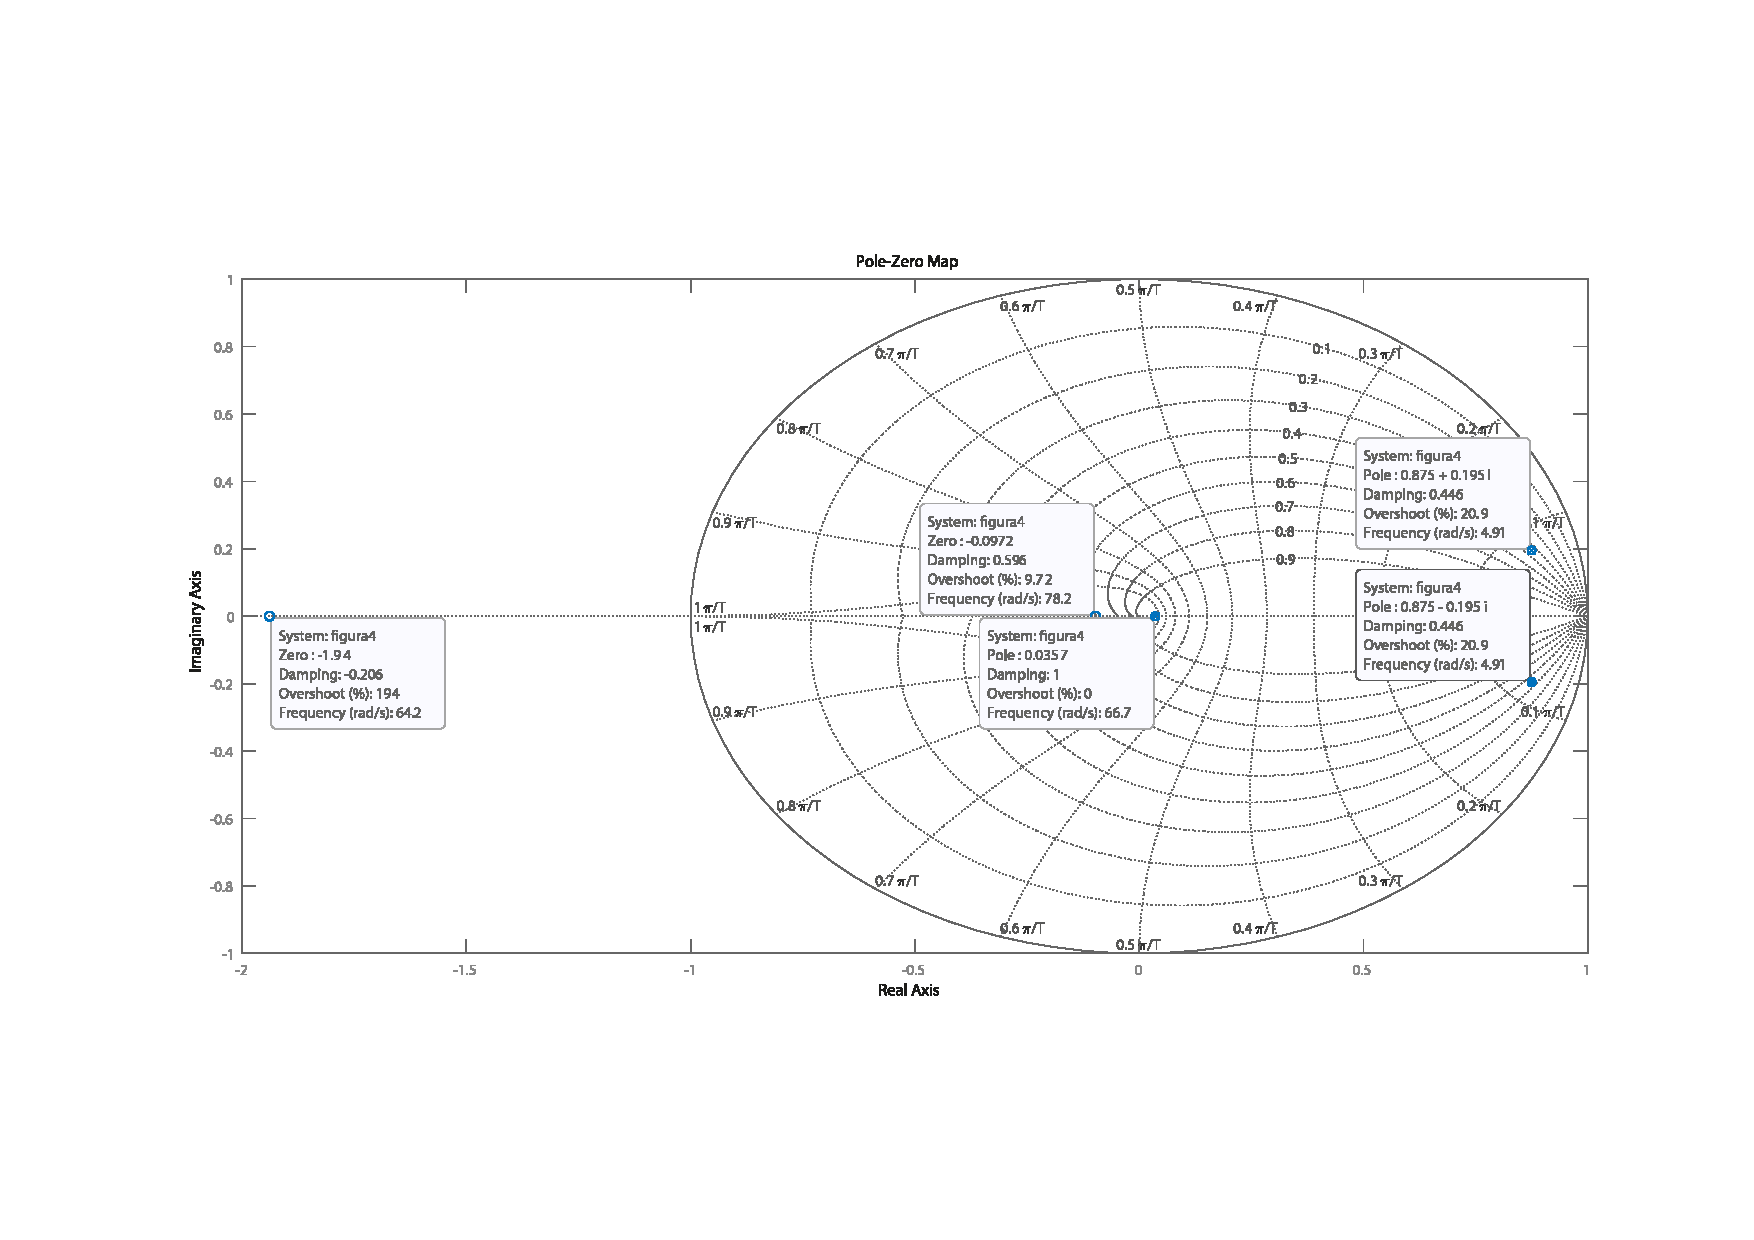
\includegraphics[clip, trim=3cm 4cm 2.8cm 4cm,
  scale=0.48]{images/figura 4.pdf}
  % izquierda,abajo,derecha,arriba
  \caption{Polos en bucle cerrado $k_a = 10$.}
    \label{fig:figura 4}
\end{figure}
}

\end{tcolorbox}%

Mediante rltool y la opción \textsc{New plot > New pole - zero map} podemos
generar una gráfica con los polos según la ganancia que colequemos en
el compensador. Los resultados son los siguientes:

\begin{itemize}
\item $k_a = 1$
  Como se puede observar en la figura \ref{fig:figura 3} los polos son:
  \begin{center}
    \begin{tabular}{ |c|c|c| } 
      \hline
      \multicolumn{3}{|c|}{Polos}\\
      \hline
      0.0393 & 0.878+0.0758$i$ & 0.878-0.0758$i$\\
      \hline
    \end{tabular}
  \end{center}
\item $k_a = 10$
  Como se puede observar en la figura \ref{fig:figura 4} los polos son:
  \begin{center}
    \begin{tabular}{ |c|c|c| } 
      \hline
      \multicolumn{3}{|c|}{Polos}\\
      \hline
      0.0218 & 0.859+0.428$i$ & 0.859-0.428$i$\\
      \hline
    \end{tabular}
\end{center}
\end{itemize}


Para el calculo de la ganancia crítica a través de la herramienta
rltool, variamos la ganancia proporcional hasta llegar al límite de la
estabilidad. 
\begin{center}
$k_{a_{\text{ganancia crítica}}}$  = 15.232
\end{center}

% Otra forma más rápida, usando el comando margin en matlab consguimos
% directamente la gananica crítica, a veces no es exacta pero podemos
% usarla como referencia.


\begin{tcolorbox}[sharp corners, colframe=bluebox, title= Ganancia crítica.]
%   $>>>$ k = margin(Gposicionz)\\
%   \vspace*{0.35em}
%   \begin{tcolorbox}[sharp corners, colback = white]
%     \color{gray}
% \begin{verbatim}
% k =
%    58.1828
% \end{verbatim}
%   \end{tcolorbox}%
    \mkanscode{
\begin{figure}[H]
  \centering
  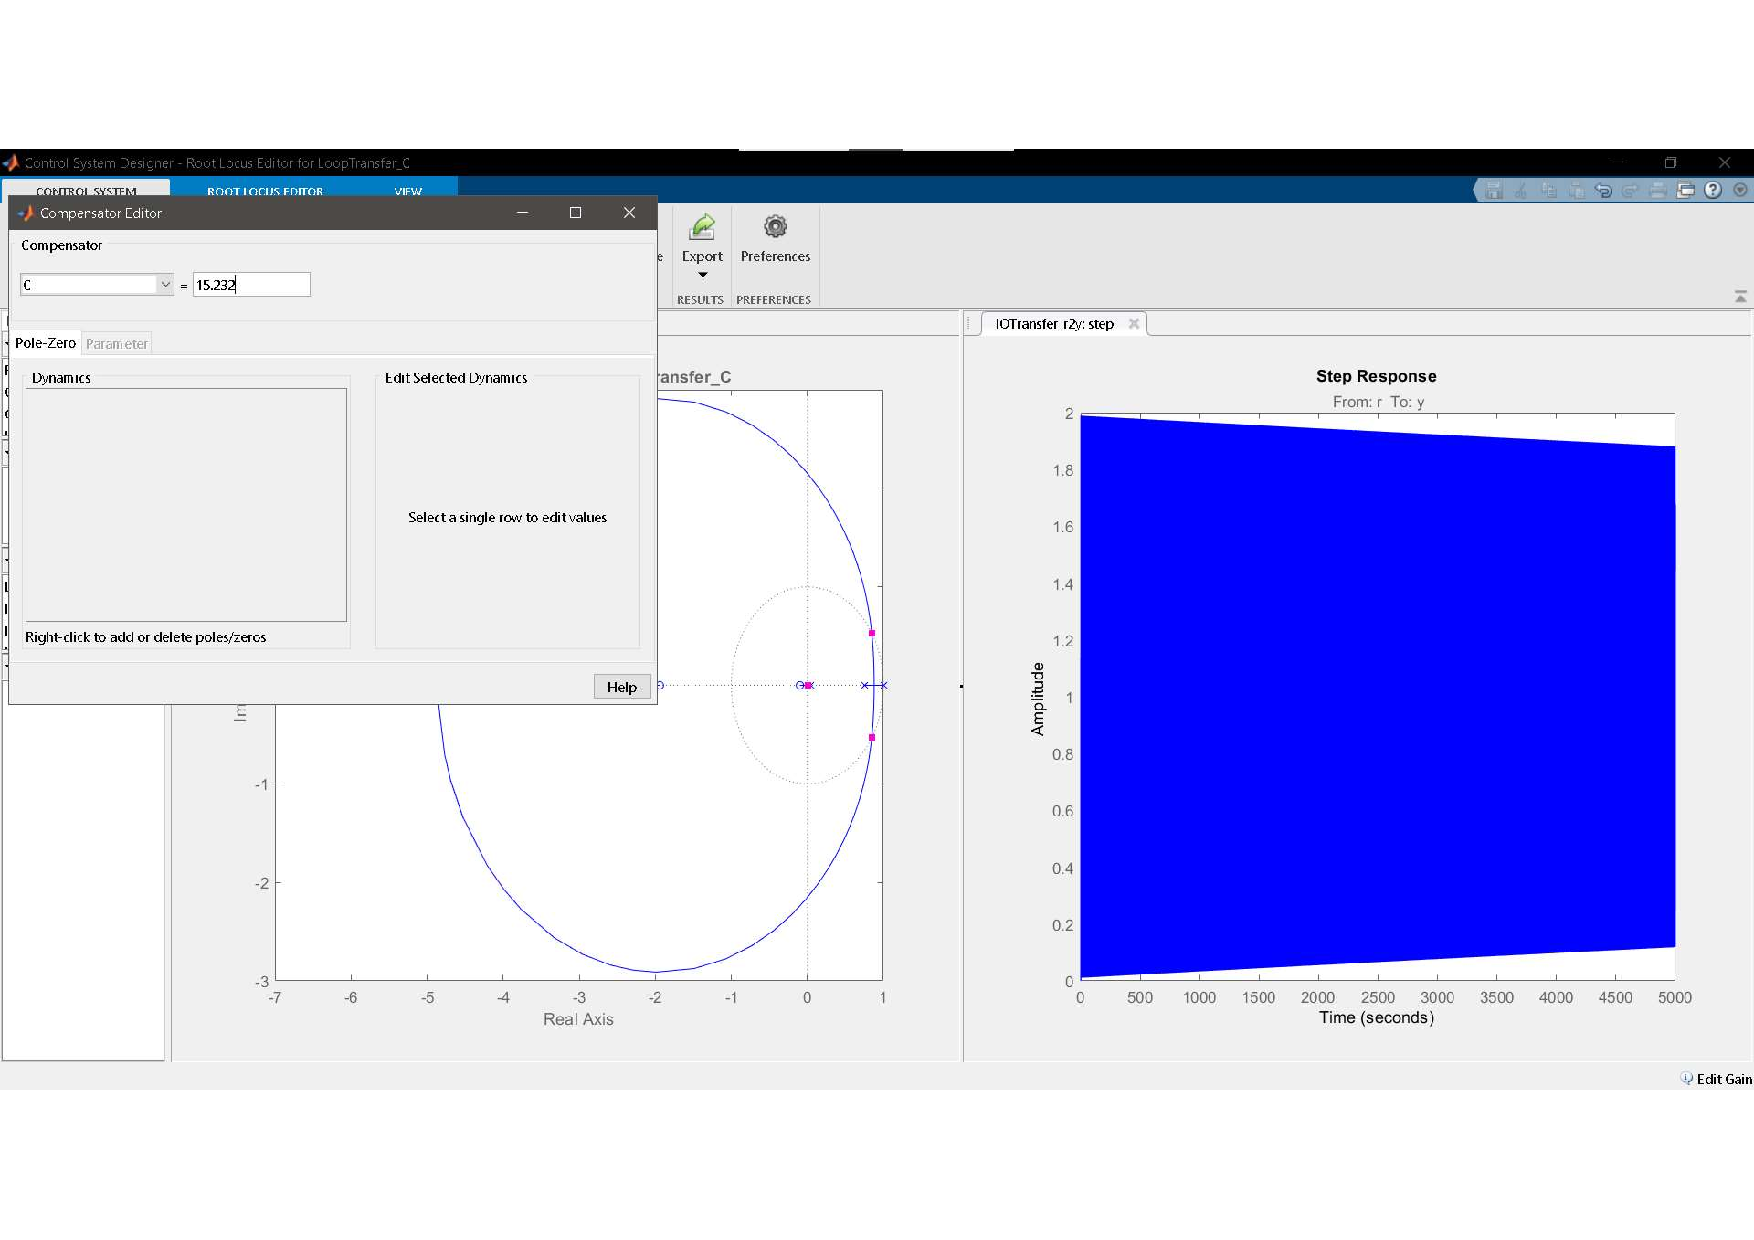
\includegraphics[clip, trim=0cm 2.5cm 0cm 2.5cm,scale=0.48]{images/figura_extra1.pdf}
  % izquierda,abajo,derecha,arriba
  \caption{Rltool - Ganancia crítica.}
    \label{fig:figura extra1}
\end{figure}
  }
\end{tcolorbox}%
